\documentclass[tikz,border=10pt]{standalone}
\usepackage{graphicx}
\usepackage{amsmath,amssymb}
\usetikzlibrary{arrows.meta, positioning, shapes.geometric, calc, fit, backgrounds}

\begin{document}
\pagecolor{white}
\newcommand{\vlabel}[1]{\rotatebox{90}{\begin{tabular}{c}#1\end{tabular}}}

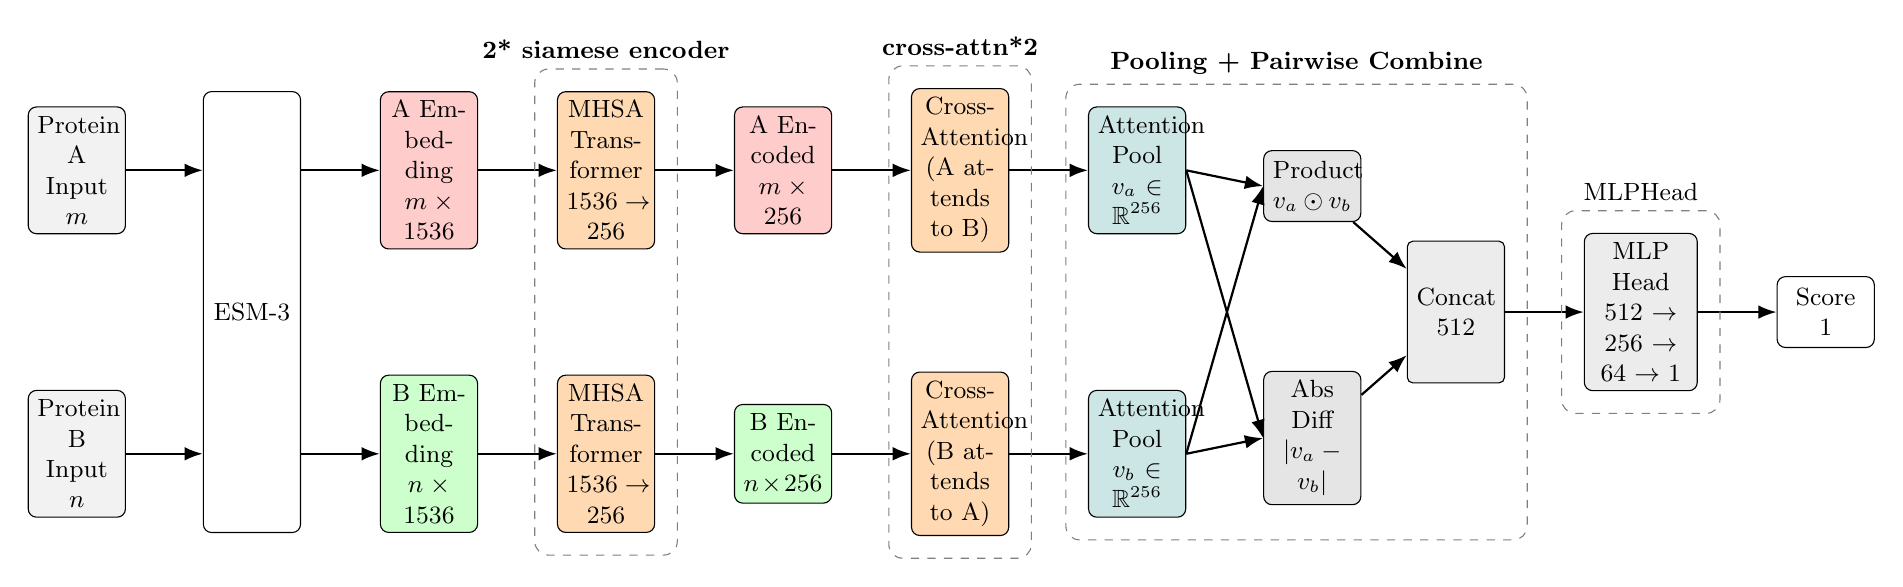
\begin{tikzpicture}[
    >=Latex,
    node distance=1.0cm and 1.4cm,
    font=\small,
    % Style definitions
    input/.style={draw, rounded corners=3pt, minimum width=1.0cm, minimum height=0.9cm, text width=1.0cm, fill=gray!10, align=center},
    esm/.style={draw, rounded corners=3pt, minimum width=1.0cm, minimum height=5.6cm, text width=1.0cm, fill=white, align=center},
    embedA/.style={draw, rounded corners=3pt, minimum width=1.0cm, minimum height=0.9cm, text width=1.0cm, fill=red!20, align=center},
    embedB/.style={draw, rounded corners=3pt, minimum width=1.0cm, minimum height=0.9cm, text width=1.0cm, fill=green!20, align=center},
    linear/.style={draw, rounded corners=3pt, minimum width=1.0cm, minimum height=0.9cm, text width=1.0cm, fill=gray!20, align=center},
    mhsa/.style={draw, rounded corners=3pt, minimum width=1.0cm, minimum height=0.9cm, text width=1.0cm, fill=orange!30, align=center},
    addnorm/.style={draw, rounded corners=3pt, minimum width=1.0cm, minimum height=0.9cm, text width=1.0cm, fill=yellow!35, align=center},
    ffn/.style={draw, rounded corners=3pt, minimum width=1.0cm, minimum height=0.9cm, text width=1.0cm, fill=blue!20, align=center},
    transformer/.style={draw, rounded corners=3pt, minimum width=1.0cm, minimum height=0.9cm, text width=1.0cm, fill=orange!30, align=center},
    crossattn/.style={draw, rounded corners=3pt, minimum width=1.0cm, minimum height=0.9cm, text width=1.0cm, fill=orange!30, align=center},
    pool/.style={draw, rounded corners=3pt, minimum width=1.0cm, minimum height=0.9cm, text width=1.0cm, fill=teal!20, align=center},
    combine/.style={draw, rounded corners=2pt, minimum width=1.0cm, minimum height=1.8cm, text width=1.0cm, fill=gray!15, align=center},
    head/.style={draw, rounded corners=3pt, minimum width=1.2cm, minimum height=0.9cm, text width=1.2cm, fill=gray!15, align=center},
    output/.style={draw, rounded corners=3pt, minimum width=1.0cm, minimum height=0.9cm, text width=1.0cm, fill=white, align=center},
    dashedbox/.style={draw, dashed, rounded corners=5pt, inner sep=8pt, gray},
    arrow/.style={->, thick, >=Latex, black},
]

% Inputs
\coordinate (inputmid) at (0,0);
\node[input, yshift=1.8cm] (protA) at (inputmid) {\vlabel{Protein A Input\\$m$}};
\node[input, yshift=-1.8cm] (protB) at (inputmid) {\vlabel{Protein B Input\\$n$}};

% ESM backbone
\node[esm, right=1.6cm of inputmid] (esm) {\vlabel{ESM-3}};

% Embeddings
\node[embedA, right=1.0cm of esm, yshift=1.8cm] (embA) {\vlabel{A Embedding\\$m \times 1536$}};
\node[embedB, right=1.0cm of esm, yshift=-1.8cm] (embB) {\vlabel{B Embedding\\$n \times 1536$}};

% MHSA transformer encoders (shared weights)
\node[transformer, right=1.0cm of embA] (trA) {\vlabel{MHSA Transformer\\$1536 \rightarrow 256$}};
\node[transformer, right=1.0cm of embB] (trB) {\vlabel{MHSA Transformer\\$1536 \rightarrow 256$}};

\node[embedA, right=1.0cm of trA] (encA) {\vlabel{A Encoded\\$m \times 256$}};
\node[embedB, right=1.0cm of trB] (encB) {\vlabel{B Encoded\\$n \times 256$}};

% Cross-attention (bidirectional)
\node[crossattn, right=1.0cm of encA] (xattA) {\vlabel{Cross-Attention\\(A attends to B)}};
\node[crossattn, right=1.0cm of encB] (xattB) {\vlabel{Cross-Attention\\(B attends to A)}};

% Attention pooling
\node[pool, right=1.0cm of xattA] (poolA) {\vlabel{Attention Pool\\$v_a \in \mathbb{R}^{256}$}};
\node[pool, right=1.0cm of xattB] (poolB) {\vlabel{Attention Pool\\$v_b \in \mathbb{R}^{256}$}};

% Combine vectors
\coordinate (poolmid) at ($(poolA)!0.5!(poolB)$);
\node[linear, right=1.6cm of poolmid, yshift=1.6cm] (prod) {\vlabel{Product\\$v_a \odot v_b$}};
\node[linear, right=1.6cm of poolmid, yshift=-1.6cm] (diff) {\vlabel{Abs Diff\\$|v_a - v_b|$}};
\coordinate (combinedmid) at ($(prod)!0.5!(diff)$);
\node[combine, right=1.2cm of combinedmid] (combine) {\vlabel{Concat\\$512$}};

% MLP head and output
\node[head, right=1.0cm of combine] (mlp) {\vlabel{MLP Head\\$512 \rightarrow 256 \rightarrow 64 \rightarrow 1$}};
\node[output, right=1.0cm of mlp] (score) {\vlabel{Score\\$1$}};

% Arrows
\draw[arrow] (protA.east) -- (esm.west |- protA.east);
\draw[arrow] (protB.east) -- (esm.west |- protB.east);
\draw[arrow] (esm.east |- embA.west) -- (embA.west);
\draw[arrow] (esm.east |- embB.west) -- (embB.west);

\draw[arrow] (embA) -- (trA);
\draw[arrow] (trA) -- (encA);
\draw[arrow] (encA) -- (xattA);

\draw[arrow] (embB) -- (trB);
\draw[arrow] (trB) -- (encB);
\draw[arrow] (encB) -- (xattB);

% Attention pooling and combine
\draw[arrow] (xattA) -- (poolA);
\draw[arrow] (xattB) -- (poolB);
\draw[arrow] (poolA.east) -- (prod.west);
\draw[arrow] (poolB.east) -- (prod.west);
\draw[arrow] (poolA.east) -- (diff.west);
\draw[arrow] (poolB.east) -- (diff.west);
\draw[arrow] (prod) -- (combine);
\draw[arrow] (diff) -- (combine);
\draw[arrow] (combine) -- (mlp);
\draw[arrow] (mlp) -- (score);

% Grouping boxes
\node[dashedbox, fit=(trA) (trB), label=above:{\textbf{2* siamese encoder}}] {};
\node[dashedbox, fit=(xattA) (xattB), label=above:{\textbf{cross-attn*2}}] {};
\node[dashedbox, fit=(poolA) (poolB) (prod) (diff) (combine), label=above:{\textbf{Pooling + Pairwise Combine}}] {};
\node[dashedbox, fit=(mlp), label=above:{MLPHead}] {};

\end{tikzpicture}

\end{document}
